\chapter{Correlation Analysis}
\label{ch:correlation}

Open from \uipth{3.\ Analysis $\to$ Correlation Analysis}.

The two-point spatial correlation function
\[
R_{uu}(\Delta x, \Delta y) = \frac{\langle u'(\mathbf{x}, t)\, u'(\mathbf{x}+\boldsymbol{\Delta}, t) \rangle}{\sigma(\mathbf{x})\,\sigma(\mathbf{x}+\boldsymbol{\Delta})}
\]
measures the degree to which velocity fluctuations at two different locations are statistically related. When $R_{uu}$ decays from 1 at $\Delta = 0$ to 0, the separation at which it crosses zero defines the integral length scale $L$, a measure of the size of the largest energy-containing eddies (Pope, 2000). The temporal autocorrelation $R(\tau)$ plays an analogous role in time, with the integral time scale $T = \int_0^{\infty} R(\tau)\,\mathrm{d}\tau$.

\noindent\textbf{Reference:} Pope, S.B. (2000). \textit{Turbulent Flows}. Cambridge University Press.

\section{Selecting a reference}

\begin{itemize}[leftmargin=1.5em]
  \item \uipth{Point mode}: left-click on the mean field to select a single reference point. Enable \uipth{$3\times3$ kernel average} to reduce sensitivity to noisy vectors at that point.
  \item \uipth{ROI mode}: left-click and drag to draw a rectangle. The correlation is computed as a spatial average over the region.
\end{itemize}

\section{Spatial correlation}

\begin{stepbox}
\begin{enumerate}[leftmargin=1.5em, topsep=2pt]
  \item Select Point or ROI mode and pick your reference on the field.
  \item Choose the velocity component: R$_{uu}$, R$_{vv}$, or R$_{ww}$.
  \item Select the \uipth{Scale method} (Table~\ref{tab:scalemethods}).
  \item Click \uipth{Compute Spatial Correlation}.
\end{enumerate}
\end{stepbox}

In Point mode you see the full 2D correlation map and two independent 1D slice panels. In ROI mode only the 1D panels are shown. The computed $L_x$ and $L_y$ are displayed in the readout strip at the bottom of the window. A vertical dashed line marks the crossing lag used by the selected scale method; for the zero-crossing method, this line is placed at the lag where $R$ first crosses zero, while $L$ is reported as the integral of $R$ up to that crossing. Click \uipth{Show Diagnostic Plot} to see the cumulative integral of $R(\Delta r)$.

\begin{figure}[htbp]
  \centering
  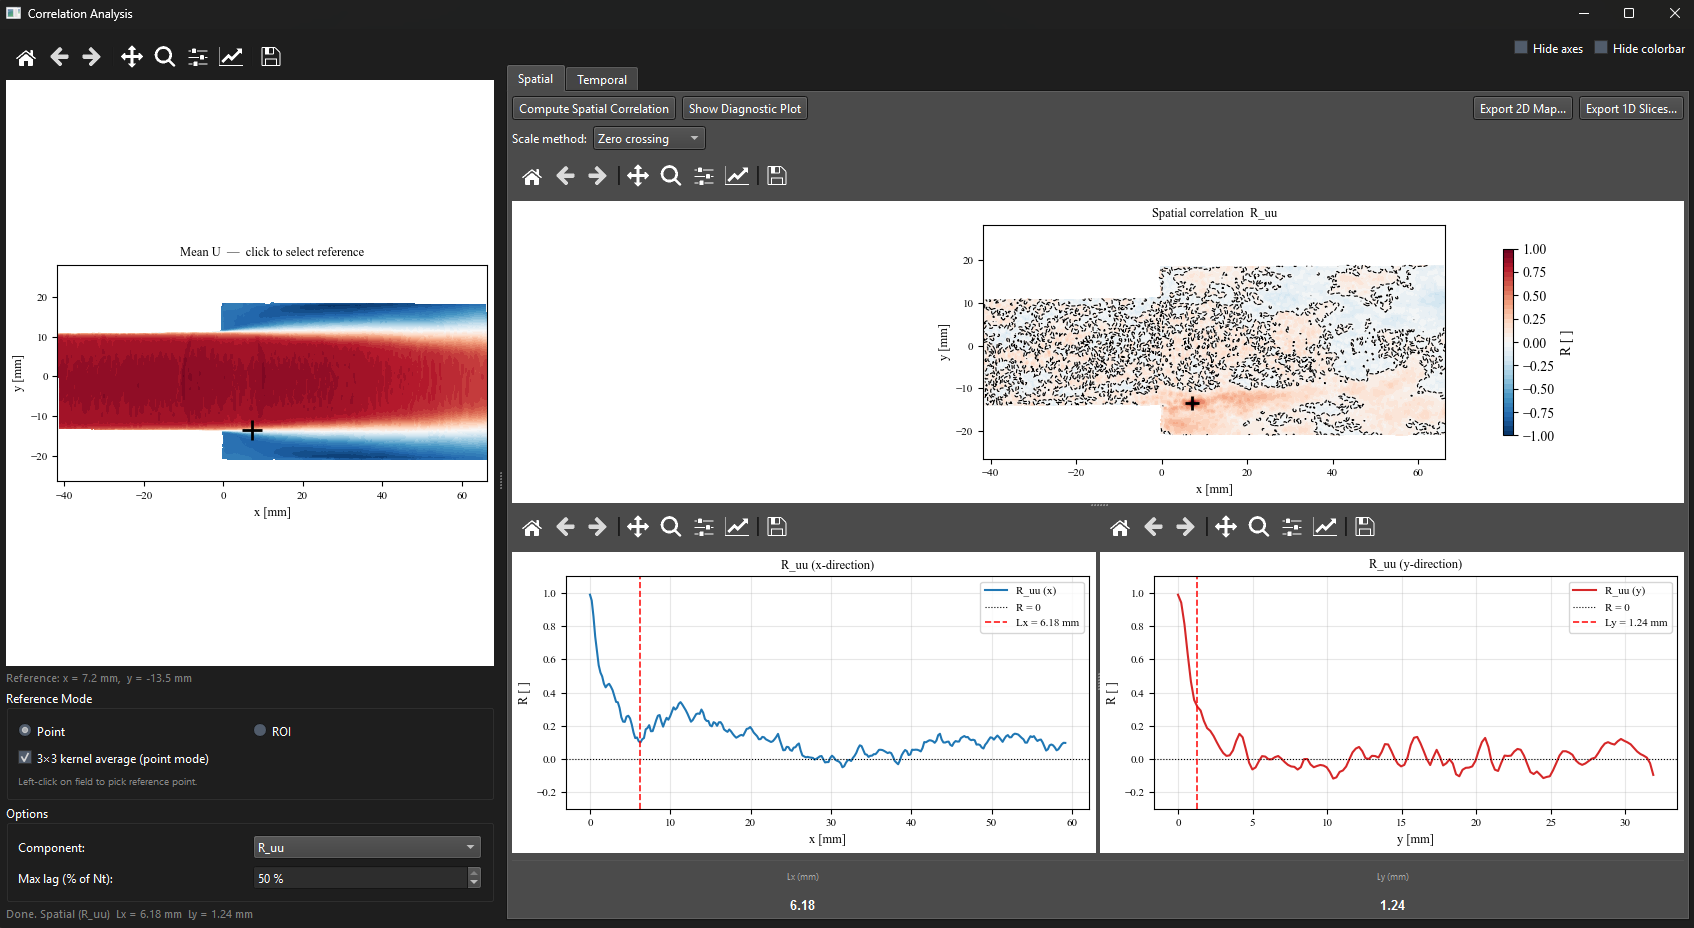
\includegraphics[width=0.92\linewidth]{fig6}
  \caption{Correlation window in ROI mode showing $R_{uu}$ in the $x$- and $y$-directions. The vertical dashed red line marks the zero-crossing lag used to compute the integral length scale. $L_x$ and $L_y$ are reported in the readout strip at the bottom.}
  \label{fig:correlation}
\end{figure}

\begin{table}[htbp]
\centering
\caption{Integral scale methods.}
\label{tab:scalemethods}
\begin{tabular}{lp{9cm}}
\toprule
\textbf{Method} & \textbf{When to use} \\
\midrule
Zero crossing   & Clean, well-resolved correlations with a clear zero crossing. Standard choice. \\
Exponential fit & Noisy correlations without a clear zero crossing. Robust to noise in the tail. \\
1/e point       & Returns the lag at which $R$ first drops to $e^{-1} \approx 0.368$ (interpolated). \\
Domain integral & When no zero crossing exists and you want a conservative upper bound. \\
\bottomrule
\end{tabular}
\end{table}

\begin{tipbox}
If unsure, start with \textbf{Zero crossing}. If the correlation does not have a clean crossing (common for low-Reynolds-number flows or short datasets), switch to \textbf{Exponential fit}.
\end{tipbox}

\section{Temporal correlation (TR only)}

\begin{stepbox}
\begin{enumerate}[leftmargin=1.5em, topsep=2pt]
  \item Click the \uipth{Temporal} tab.
  \item Pick a reference point or draw an ROI as before.
  \item Set \uipth{Max lag (\% of Nt)}: 50\% is usually sufficient.
  \item Select the Scale method.
  \item Click \uipth{Compute Temporal Correlation}.
\end{enumerate}
\end{stepbox}

Results show $R(\tau)$ vs time lag $\tau$ in milliseconds, with integral time scale $T$ and Taylor microscale $\lambda_t$ marked.

\section{Multi-case comparison}

Spatial 1D slice and temporal correlation curves support CSV import and overlay (Chapter~\ref{ch:multicase}).

% ============================= CHAPTER 10 ==============================
